\chapter{Mankiw微观经济学笔记}

\section{经济学十大原理}

\subsection*{人们面临权衡取舍}

最常见的取舍在于对资源的分配, 另一种取舍在于如何平衡效率(社会能从稀缺资源中得到最大利益)与平等(经济成果在社会成员中平均分配). 

\subsection*{机会成本原理}

机会成本, 即为了得到某种东西而必须放弃的东西. 用粗糙的数学视角来看, 就是说在选择$A_1,\cdots ,A_n$之间存在一个关联$f$, 使得$f(A_1,\cdots ,A_n)$为定值$0$. 

\begin{example}{生产可能性边界}
	考虑一个电脑-汽车生产的模型. 在这个模型中, 让生产电脑的工人转而生产汽车, 将会导致汽车产量增加和电脑产量下降, 反之亦然. 因此, 我们可以用电脑产量作为机会成本来描述汽车产量. 
	\begin{figure}[H]
		\centering
		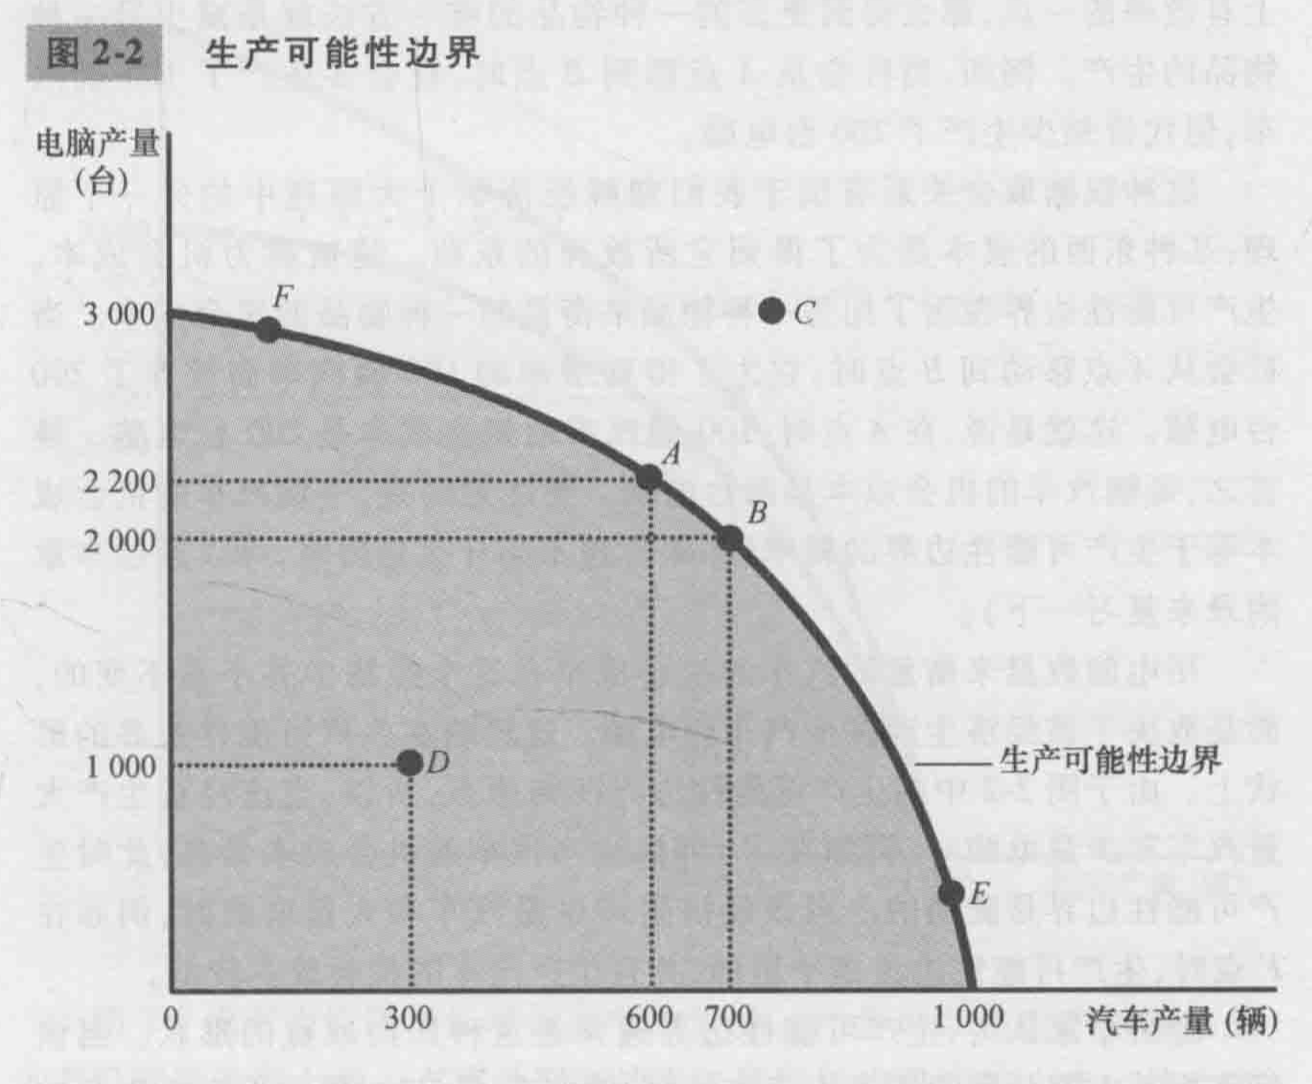
\includegraphics[width=8cm]{attachment/Fig2_2.png}
	\end{figure}
	从数学的视角来看, 两种产量$A_1,A_2$具有类似$A_1+A_2=C$的关系. 特别地, 极端追求汽车产量会让大量熟练于电脑生产的工人转而生产汽车, 这时付出很多电脑工人也只能推动汽车产量的微小变化, 因此越靠近$E$点, 一单位汽车所对应的电脑成本越高. 即是说整个曲线呈现上凸的形状. 
\end{example}

\subsection*{理性人考虑边际量}

实际上, 这个原理基于某种公设, 即所谓理性人(经济人)假设: \textit{人们总是以理性和利己的行为追求目标利益最大化}. 

用数学的话, 考虑一个将行为变成结果的函数$f$. 为了让$f(x)$取得最大值$M$, 可以先找到那些使得$f(x)$与$M$差距不大的$x$, 再在这些$x$(边际量)中找到$f(x)=M$的点. 

\begin{example}{沉没成本}
	已经付出且不可收回的成本, 就成为沉没成本. 按照边际分析的原理, 理性人不应当考虑沉没成本, 因为此时再付出多少都与沉没成本无关. (当然这是在不考虑个人情绪价值等的情况下)
\end{example}

\subsection*{人们会对激励做出反应}

在分析经济行为的后果时, 不仅要考虑其本身直接后果, 还要考虑其作为激励的影响. 

\begin{example}{关于弹性的直观认知}
	提高价格的确能增加生产者的单件收入, 但这会导致消费者的购买量减少, 总收益不一定增加. 实际上, 当需求弹性较小时收益会增加. 
\end{example}

\subsection*{比较优势原理: 贸易可以使每个人的状况都变得更好}

当贸易的两者各具有一方面的特长时, 贸易的优势是显然的. 实际上, 当其中一者具有绝对性优势时, 贸易也会带来改善. 例如, 回到例1.1的情景, 如果两个工厂$A_1,A_2$都开设电脑-汽车的生产线, 即使$A_2$的生产可能性边界较$A_1$更向外(即具有两方面的优势), 在它们之间必有其一生产汽车的机会成本更小, 同时(因为只有两种产物)其生产电脑的机会成本更大. 

因此, 贸易可以让每个人都从事自己最擅长(具有比较优势)的活动, 从而改善所有人的状况. 

\subsection*{市场通常是组织经济活动的好方法}

在后面我们会分析, 利用市场达到供给-需求均衡, 会使市场总收益最大化. 

\subsection*{政府有时可以改善市场结果}

政府需要保证市场的正常开展、避免或补救市场失灵(市场本身无法有效配置资源, 例如出现垄断、发生灾害等)、保证某种平等. 

\subsection*{一国的生活水平取决于它生产物品与服务的能力}

\subsection*{当政府发行了过多货币时, 物价上升}

\subsection*{社会面临通货膨胀与失业之间的短期权衡取舍}

\newpage
\section{分析市场运行的基本工具}

所谓市场, 即是由某种物品或服务的买者和卖者组成的一个群体. 为了构建理想化的模型, 我们总是考虑\textit{(完全)竞争市场}: 买者和卖者的数量足够多、商品之间的差异足够小以至于每个人对价格的影响都是微乎其微的. 之后会介绍如何在完全竞争市场模型的基础上进行针对税收、垄断等的分析. 

\subsection{需求与供给}

1. \textit{需求量}: 买者愿意并且能够购买的一种物品的数量. 在考虑需求对价格的反应时, 人们一般会在价格上升时减少自己的需求量(这被称作\textit{需求定理}). 我们可以用大致的线性关系图像来表达这一定理. 其中, 随着价格的变化而改变的需求量称作\textit{在曲线上的移动}, 不同于\textit{将整个曲线进行移动}. 这意味着我们总有两种方式改变需求量: 变动价格或给予激励. 

\begin{figure}[H]
	\centering
	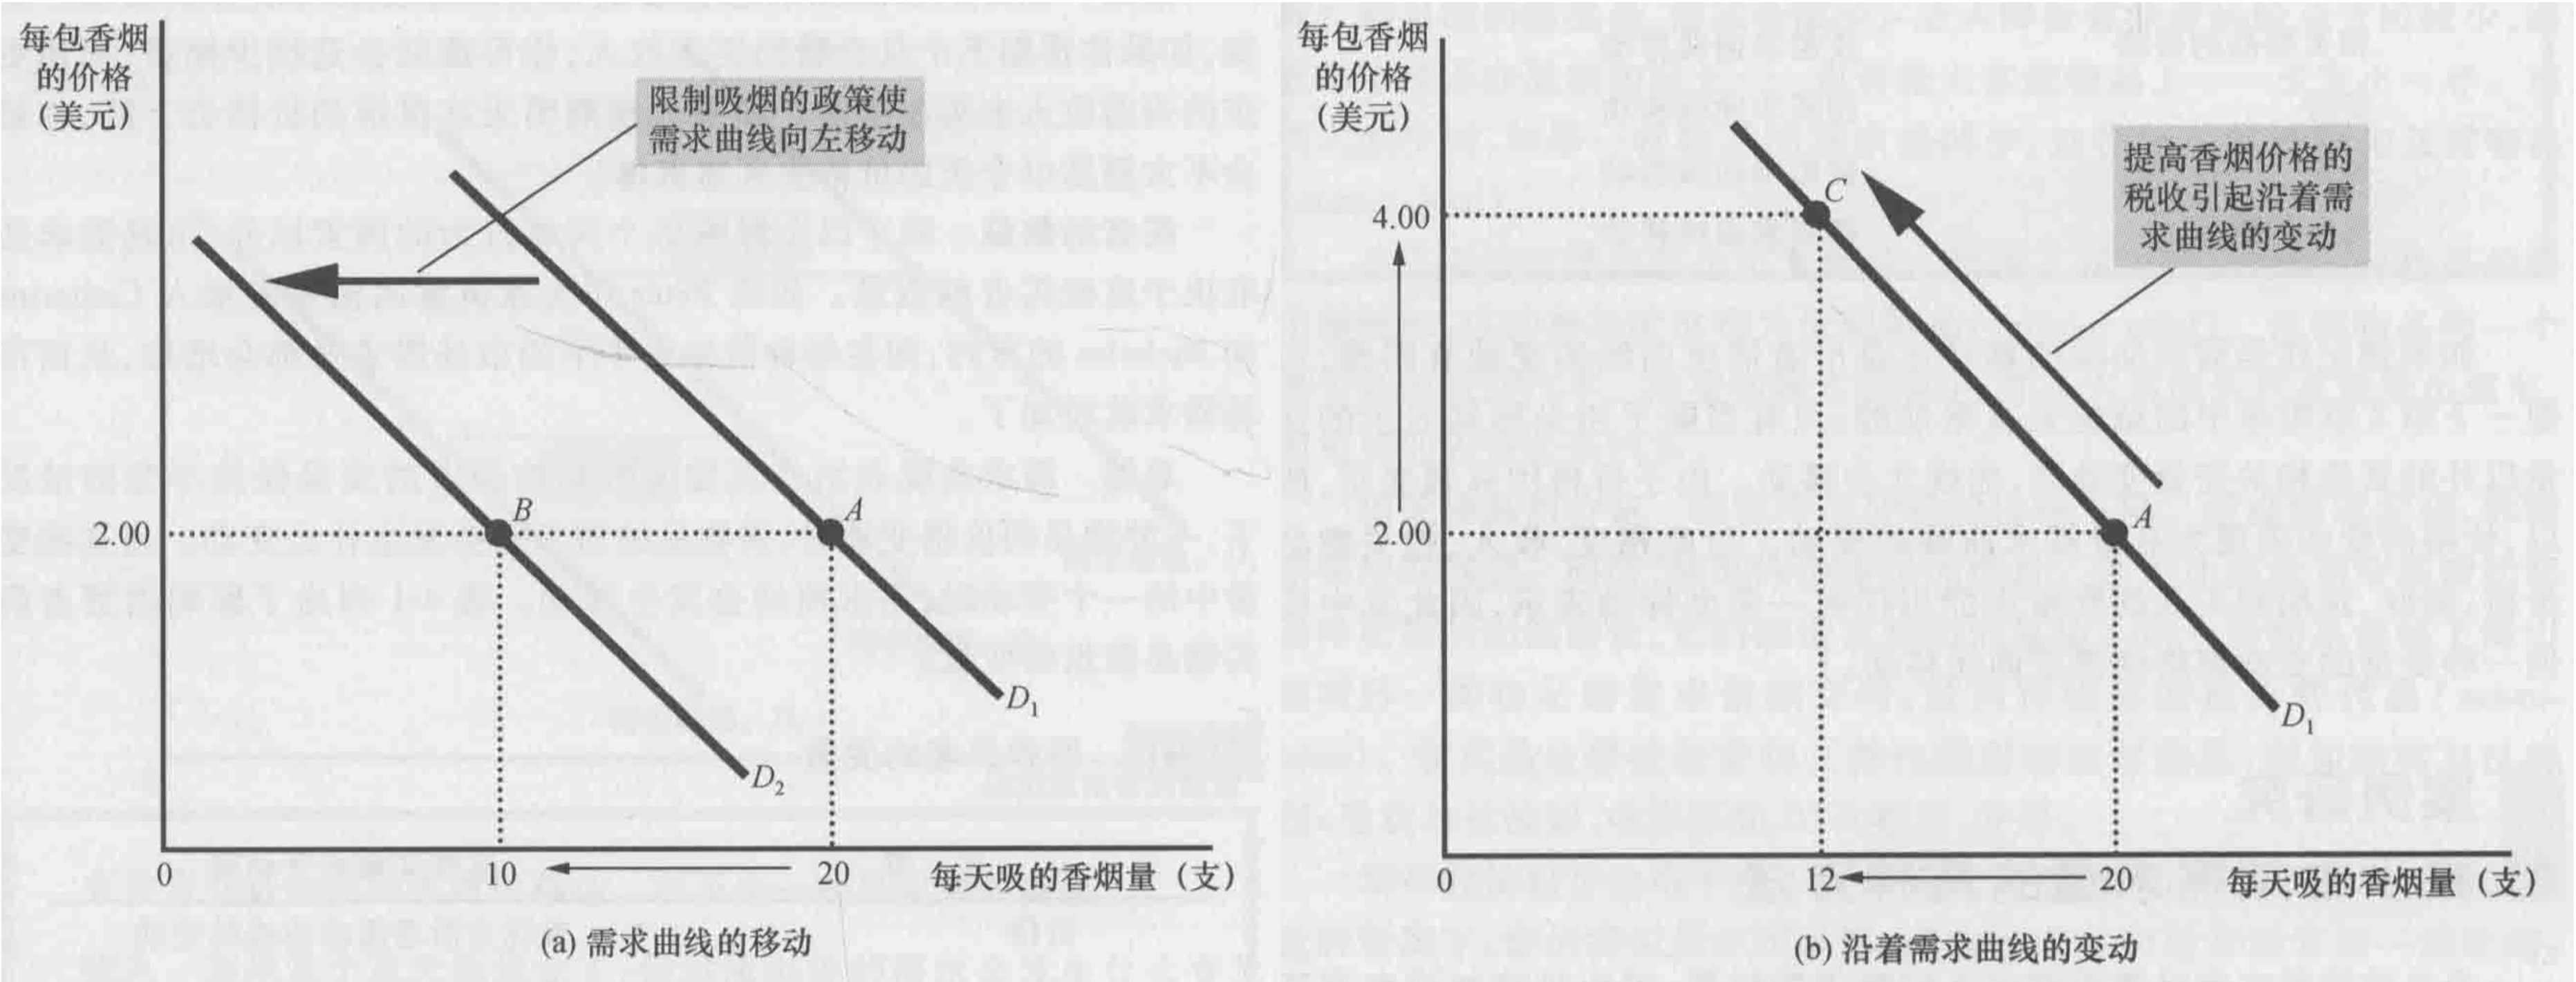
\includegraphics[width=18cm]{attachment/Fig4_2.png}
\end{figure}

与需求曲线移动相关的量: 收入(高档物品, 低档物品), 相关物品的价格(替代品, 互补品), 偏好, 预期, 相关激励等等. 

2. \textit{供给量}: 卖者愿意并且能够出售的该种物品的数量. 类似于需求, 我们有\textit{供给定理}: 一种物品价格上升, 其供给量增加. 

\begin{figure}[H]
	\centering
	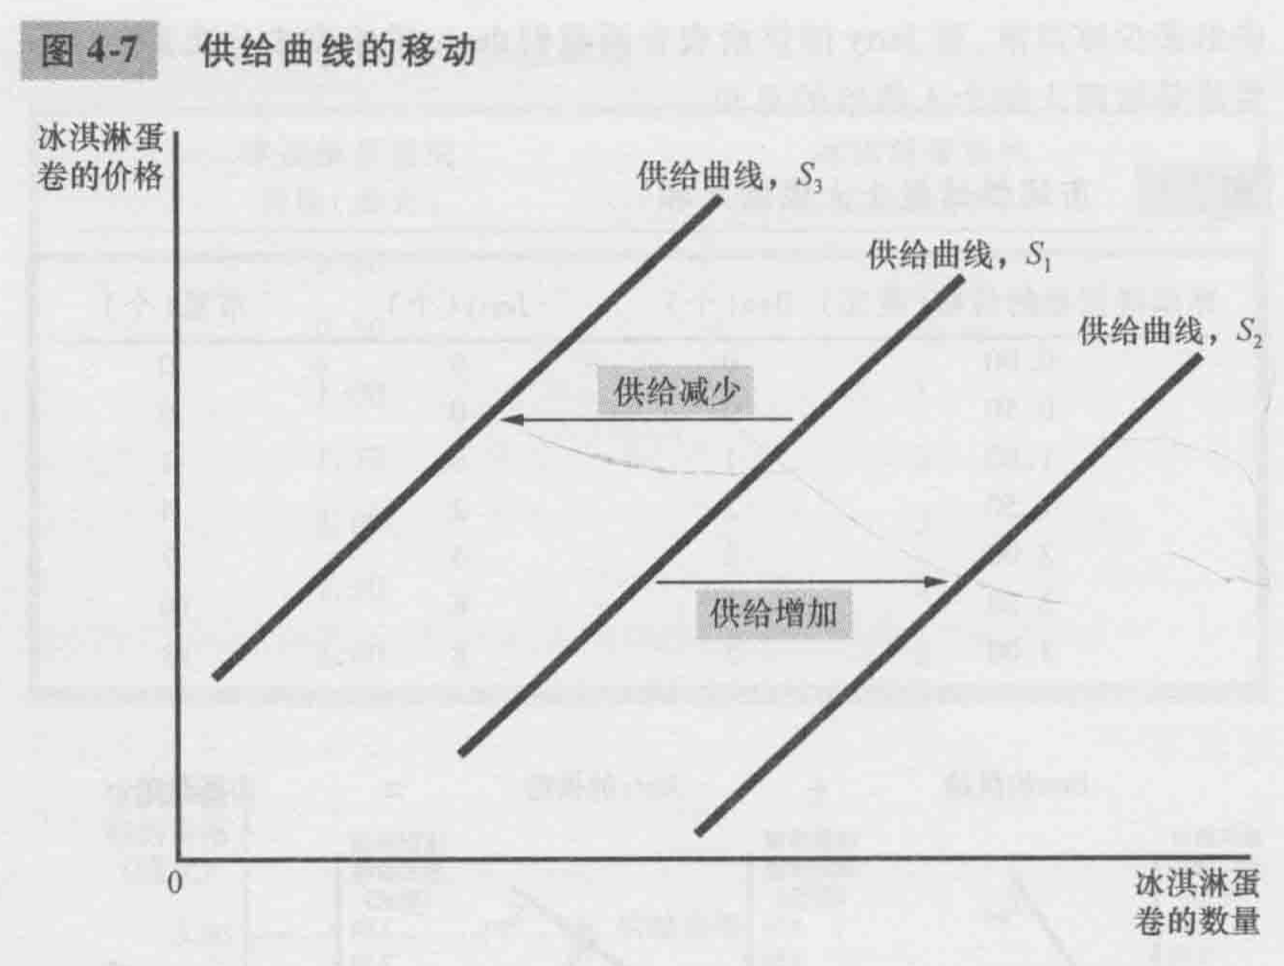
\includegraphics[width=8cm]{attachment/Fig4_7.png}
\end{figure}

与供给曲线移动相关的量: 成本, 技术, 预期, 相关激励等. 

3. 市场的需求曲线与供给曲线: 实际上, 每个消费者/生产者对价格的变化并不一定敏感, 因此个人需求/供给曲线不一定是一条直线. 然而, 由于市场上存在大量消费者/生产者, 可以认为市场的需求/供给曲线是光滑的. 

\subsection{市场均衡}

将(市场)供给曲线与需求曲线画在一张图上. 当供给曲线与需求曲线相交的时候, 就称达到了\textit{均衡}. 当供给大于需求时, 称为\textit{过剩}. 需求大于供给时, 称为\textit{短缺}. 当市场处于不均衡的状态时, 例如过剩, 此时生产者有货物积压, 他们自然地会降低价格以将货物售出, 于是逐渐达到均衡状态. 这被称作\textit{供求定理}. 另外, 我们稍后会具体分析, 为什么均衡能使得消费者和生产者的利益同时最大化. 



\subsection{弹性}



